\documentclass[12pt,a4paper]{article}

\usepackage[utf8]{inputenc}
\usepackage[T1]{fontenc}
\usepackage[spanish]{babel}
\usepackage{geometry}
\usepackage{array}
\usepackage{longtable}
\usepackage{graphicx}
\usepackage{enumitem}

\geometry{margin=2.5cm}
\renewcommand{\arraystretch}{1.4}
\setlength{\parindent}{0pt}
\setlength{\parskip}{6pt}

\begin{document}

\begin{center}
{\large \textbf{Transcripción de la evaluación escrita a mano}}\\[2pt]
EV-PRAC-01 -- Ingeniería de Requerimientos (ISR-401)
\end{center}

Esta es la transcripción fiel de la prueba escrita a mano el 18 de noviembre de 2026; las fotografías de las hojas están en el anexo.

\hrule
\vspace{6pt}

% ================= HOJA 1 =================
\textbf{Hoja 1}

Ing - Req Evaluación Parcial.\hfill Nombre: Jordan Basurto.

18-11-2026

4 tarea

T1

(a) Explique con sus palabras que es un requisito segun ISO/IEC/IEEE y Con esa explicación, decida si E7 y E12 son requisitos del producto FRIOVAC.

Un requisito es una condición que se debe cumplir antes de Construir el software definir lo Que se va a hacer.

E7 no es un requisito del producto Friovac porque es una acción que se hace Fuera del sistema.

E12 no es un requisito y que es un plan de proyecto el cual se planificará mediante una entrevista

(b) Explique qué describe la planificación de requisitos de los Interesados (STRS), la especificación de requisitos del sistema (SyRS) y la especificación de requisitos del software (SRS) en este proyecto. Para cada una de un enunciado del insumo A que diría en ella y por qué

\begin{itemize}[noitemsep]
\item STRS --- lo que necesitan y esperan los interesados --- E1
\item Sy RS --- lo que debe cumplir FRIOVAC como sistema --- E6
\item SRR --- lo que debe hacer y cumplir la Plataforma web. (Software). --- E8.
\end{itemize}

\newpage
% ================= HOJA 2 =================
\textbf{Hoja 2}

Para cada hecho H1 a H5 indique a qué Actividad del Proceso IR corresponde

\begin{center}
\begin{tabular}{|l|l|l|}
\hline
Hn & Act Proceso & Marco de Pohl \\
\hline
H1 & Elicitacion & Central \\
\hline
H2 & Análisis y Negociación & Central \\
\hline
H3 & Especificacion & Central \\
\hline
H4 & Validacion & Central \\
\hline
H5 & Gestión & Transversal \\
\hline
\end{tabular}
\end{center}

T2 Clasificación y auditoría - a.

\begin{center}
\begin{tabular}{|l|p{3.4cm}|l|p{5.2cm}|}
\hline
ID & Tipo & \multicolumn{2}{l|}{Documento y Justificación} \\
\hline
E1 & Funcional & STRS & Necesidad del interesado \\
\hline
E2 & Req. de Dominio & STRS & Regla de norma térmica \\
\hline
E3 & Restricción & Sy Rs & Impone un sensor \\
\hline
E4 & Restricción (de Proyecto) & STRS & El plazo y El costo \\
\hline
E5 & Funcional & SRS & Función de software. \\
\hline
E6 & No Funcional & Sy RS & Seguir operando durante cortes \\
\hline
E7 & No es Requisito. & \multicolumn{2}{l|}{Ninguno, se Registro como contexto} \\
\hline
E8 & No funcional & SRS & Eficiencia y manejo de Velocidad \\
\hline
E9 & Restricción & SRS & Compatibilidad y Portabilidad. \\
\hline
E10 & No funcional & SRS & limita quien Registra Acciones \\
\hline
E11 & No funcional & SRS & Mide que tan faciles son las pantallas para aprender \\
\hline
E12. & Req de Proceso & \multicolumn{2}{p{7.2cm}|}{Ninguno: se registro como Plan de proyeccto. define como hacer la elicitacion y quien firma.} \\
\hline
\end{tabular}
\end{center}

\newpage
% ================= HOJA 3 =================
\textbf{Hoja 3}

b. Auditoria

\begin{center}
\small
\begin{tabular}{|l|p{2.6cm}|p{2.6cm}|p{2.2cm}|p{2.6cm}|}
\hline
ID & Termino o problematico & Característica 29148 & Propiedad SMART & Justif. \\
\hline
B1 & Ambiguedad, no es medible & Verificable y Singular & Measurable & No tiene umbral \\
\hline
B2 & Sin destinatorio & Inequivoco y Completo & Specific & No fija plazo \\
\hline
B3 & «En todo momento.» & Fiable & Attainable & Sin energia no se puede Registrar \\
\hline
B4 & «MongoDB alojada en la nube» & Apropiado y Necesario & traceable & Opcional \\
\hline
B5 & «Si es posible» & Verificable e Inequivoco & Specific & Opcional \\
\hline
B6 & Ninguno, esto bien formado &  & Ninguna. & Esta bien formado. \\
\hline
\end{tabular}
\end{center}

T3 Redacción de requisitos bien formados.

6 Req bien formados

\newpage
\section*{Anexo: fotografías de las hojas}

\begin{center}
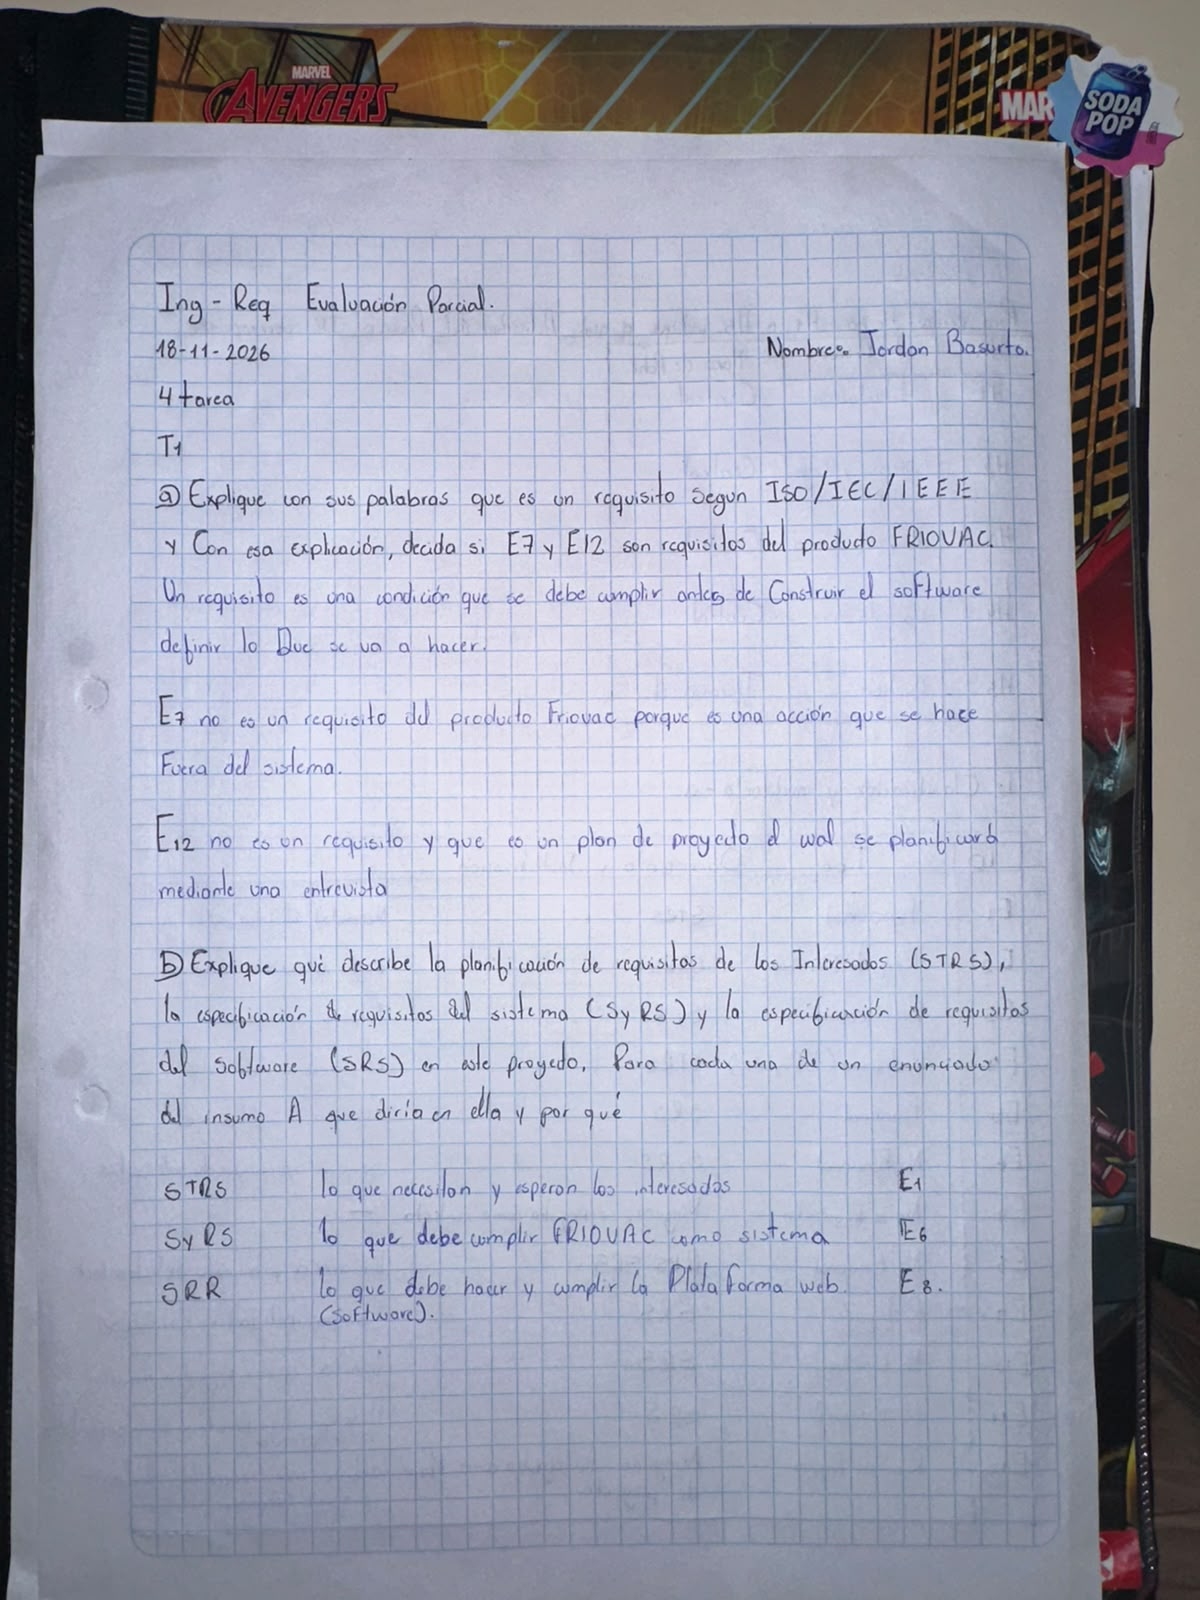
\includegraphics[width=0.85\textwidth,height=0.85\textheight,keepaspectratio]{evidencias/hoja-01.jpg}\\[4pt]
Hoja 1
\end{center}
\newpage
\begin{center}
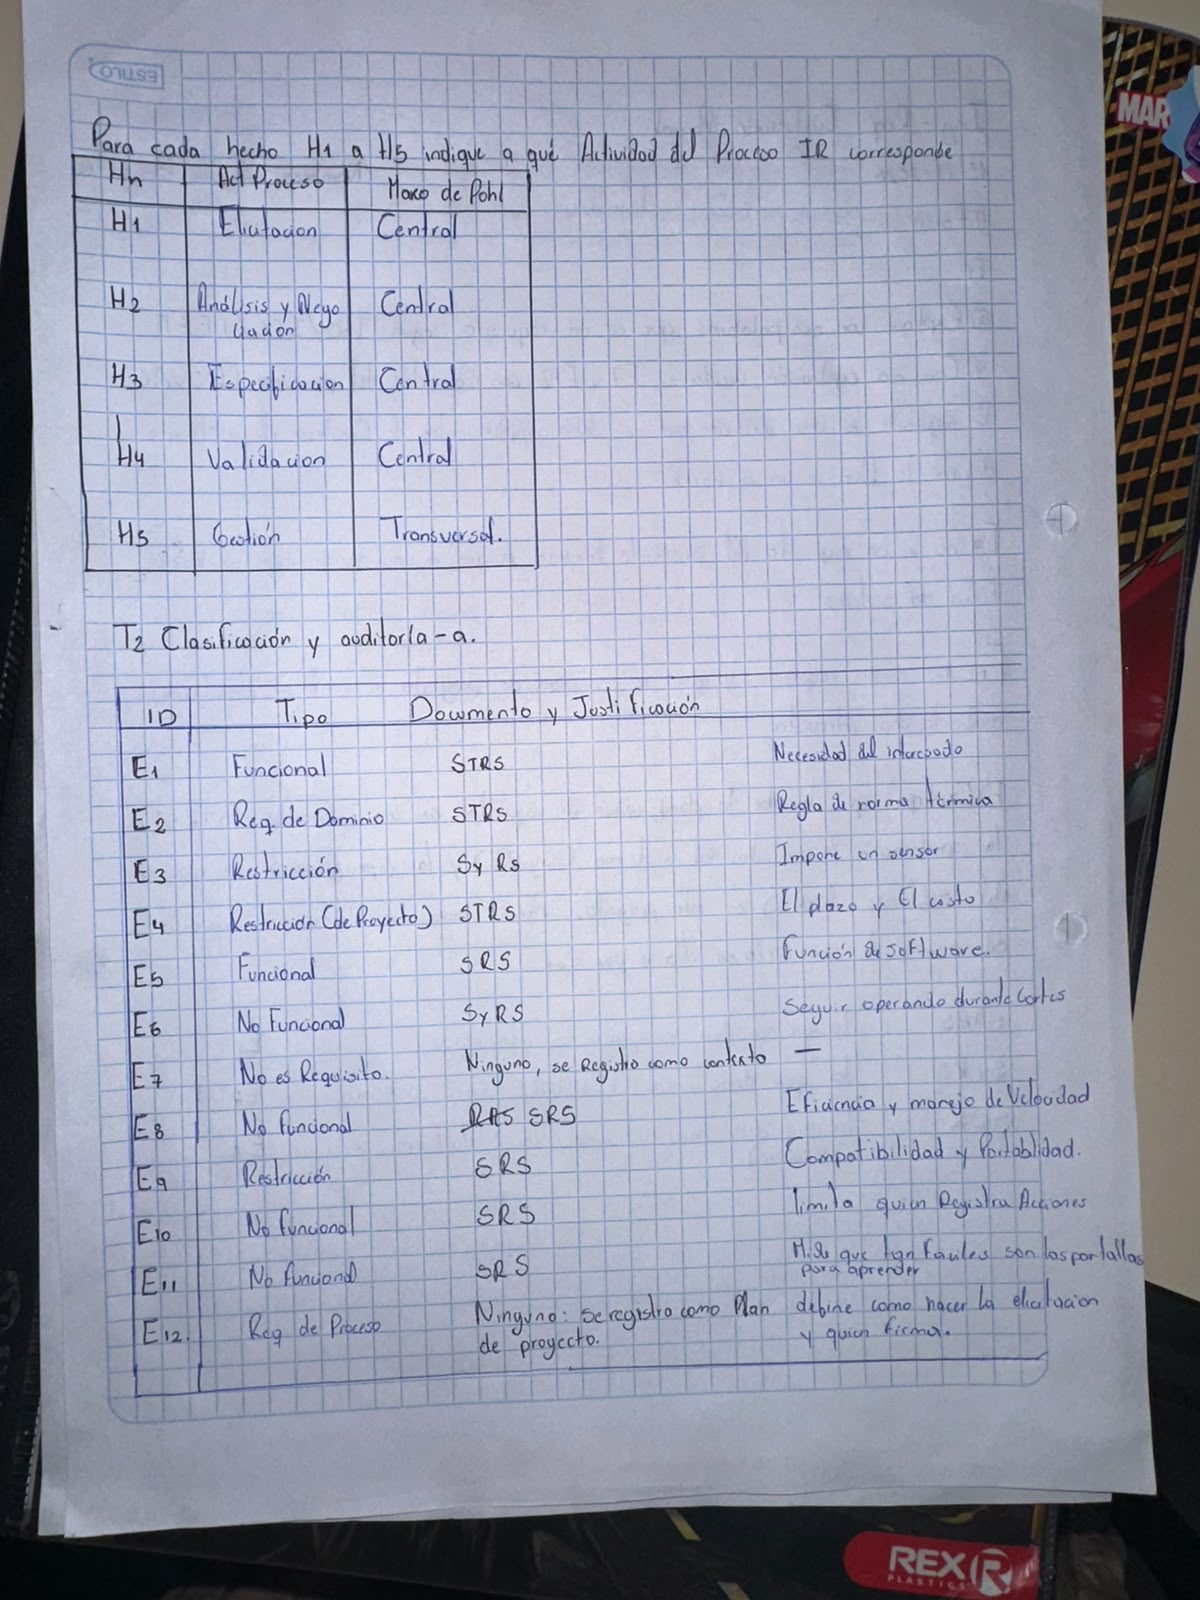
\includegraphics[width=0.85\textwidth,height=0.85\textheight,keepaspectratio]{evidencias/hoja-02.jpg}\\[4pt]
Hoja 2
\end{center}
\newpage
\begin{center}
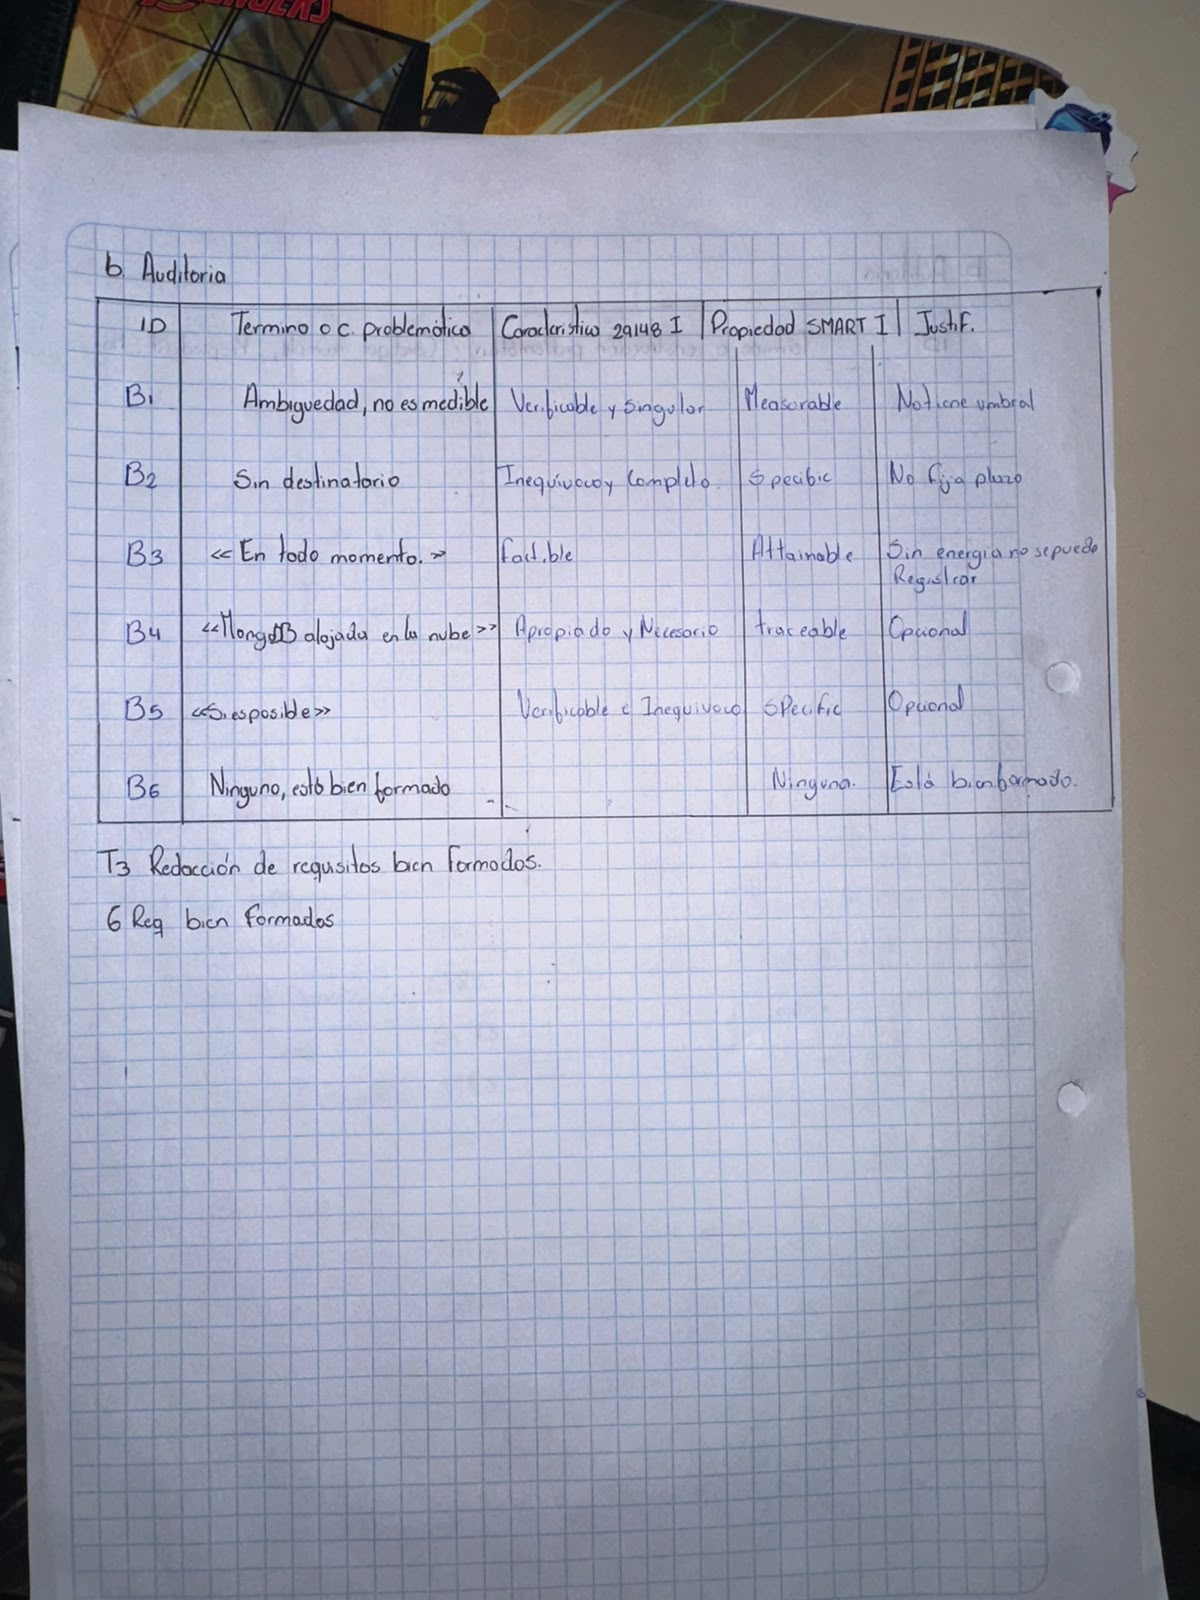
\includegraphics[width=0.85\textwidth,height=0.85\textheight,keepaspectratio]{evidencias/hoja-03.jpg}\\[4pt]
Hoja 3
\end{center}

\end{document}
